%%%%%%%%%%%%%%%%%%%%%%%%%%%%%%%%%%%%%%%%%
% Journal Article
% LaTeX Template
% Version 1.4 (15/5/16)
%
% This template has been downloaded from:
% http://www.LaTeXTemplates.com
%
% Original author:
% Frits Wenneker (http://www.howtotex.com) with extensive modifications by
% Vel (vel@LaTeXTemplates.com)
%
% License:
% CC BY-NC-SA 3.0 (http://creativecommons.org/licenses/by-nc-sa/3.0/)
%
%%%%%%%%%%%%%%%%%%%%%%%%%%%%%%%%%%%%%%%%%

%----------------------------------------------------------------------------------------
%	PACKAGES AND OTHER DOCUMENT CONFIGURATIONS
%----------------------------------------------------------------------------------------

\documentclass[twoside,twocolumn]{article}

\usepackage{blindtext} % Package to generate dummy text throughout this template 

\usepackage[sc]{mathpazo} % Use the Palatino font
\usepackage[T1]{fontenc} % Use 8-bit encoding that has 256 glyphs
\linespread{1.05} % Line spacing - Palatino needs more space between lines
\usepackage{microtype} % Slightly tweak font spacing for aesthetics

\usepackage[english]{babel} % Language hyphenation and typographical rules

\usepackage[hmarginratio=1:1,top=32mm,columnsep=20pt]{geometry} % Document margins
\usepackage[hang, small,labelfont=bf,up,textfont=it,up]{caption} % Custom captions under/above floats in tables or figures
\usepackage{booktabs} % Horizontal rules in tables

\usepackage{lettrine} % The lettrine is the first enlarged letter at the beginning of the text

\usepackage{enumitem} % Customized lists
\setlist[itemize]{noitemsep} % Make itemize lists more compact

\usepackage{abstract} % Allows abstract customization
\renewcommand{\abstractnamefont}{\normalfont\bfseries} % Set the "Abstract" text to bold
\renewcommand{\abstracttextfont}{\normalfont\small\itshape} % Set the abstract itself to small italic text

\usepackage{titlesec} % Allows customization of titles
\renewcommand\thesection{\Roman{section}} % Roman numerals for the sections
\renewcommand\thesubsection{\roman{subsection}} % roman numerals for subsections
\titleformat{\section}[block]{\large\scshape\centering}{\thesection.}{1em}{} % Change the look of the section titles
\titleformat{\subsection}[block]{\large}{\thesubsection.}{1em}{} % Change the look of the section titles

\usepackage{fancyhdr} % Headers and footers
\pagestyle{fancy} % All pages have headers and footers
\fancyhead{} % Blank out the default header
\fancyfoot{} % Blank out the default footer
\fancyhead[C]{Running title $\bullet$ May 2016 $\bullet$ Vol. XXI, No. 1} % Custom header text
\fancyfoot[RO,LE]{\thepage} % Custom footer text

\usepackage{titling} % Customizing the title section

\usepackage{hyperref} % For hyperlinks in the PDF

% Packages maison
\usepackage{amsmath,amssymb} % For including math equations, theorems, symbols, etc
\usepackage{bm}
\usepackage{graphicx} % Required for including images
\graphicspath{{../Figures/}} % Set the default folder for images
\usepackage{prettyref}

%----------------------------------------------------------------------------------------
%	TITLE SECTION
%----------------------------------------------------------------------------------------

\setlength{\droptitle}{-4\baselineskip} % Move the title up

\pretitle{\begin{center}\Huge\bfseries} % Article title formatting
\posttitle{\end{center}} % Article title closing formatting
\title{A database of piano and orchestral midi scores.\\Application to automatic projective orchestration} % Article title
\author{%
\textsc{John Smith}\thanks{A thank you or further information} \\[1ex] % Your name
\normalsize University of California \\ % Your institution
\normalsize \href{mailto:john@smith.com}{john@smith.com} % Your email address
%\and % Uncomment if 2 authors are required, duplicate these 4 lines if more
%\textsc{Jane Smith}\thanks{Corresponding author} \\[1ex] % Second author's name
%\normalsize University of Utah \\ % Second author's institution
%\normalsize \href{mailto:jane@smith.com}{jane@smith.com} % Second author's email address
}
\date{\today} % Leave empty to omit a date
\renewcommand{\maketitlehookd}{%
\begin{abstract}
\noindent This article introduces the \textbf{NAME} dataset, a freely-available collection of midi scores 

midi score database. It is composed by (137 OU 224 si IMSLP, mais c'est tout faux) pairs of one piano score and one corresponding orchestration. To our best knowledge, this is the first database of this kind. Thus, we also introduce a projective orchestration task, which roughly consists in learning to perform automatic orchestration of a piano score. This task can be addressed using learning methods on this database.  
\end{abstract}
}

%----------------------------------------------------------------------------------------

\begin{document}

% Print the title
\maketitle

%----------------------------------------------------------------------------------------
%	ARTICLE CONTENTS
%----------------------------------------------------------------------------------------

\section{Introduction}
% Orchestration = definition
Orchestration is the subtle art of writing musical pieces for the orchestra by combining the properties of various instruments in order to achieve a particular sonic rendering. \cite{koechli_orch,Rimsky-Korsakov:1873aa}.
Several treatise of orchestration exist \textbf{CITE}, but they all consist in a sum of example, and it seems that it has not been possible yet to theoretize.
One reason might be because orchestration involve complexes psycho-acoustic mechanisms and embodies a huge complexity.
EXPLIQUER PUORQUOI ???
Hence, we believe that a thorough scientific investigation of the orchestration could help the advance of the discipline and help understanding the mechanisms involved.
but no scientific investigation has been thoroughly lead.

\begin{figure}
\centering
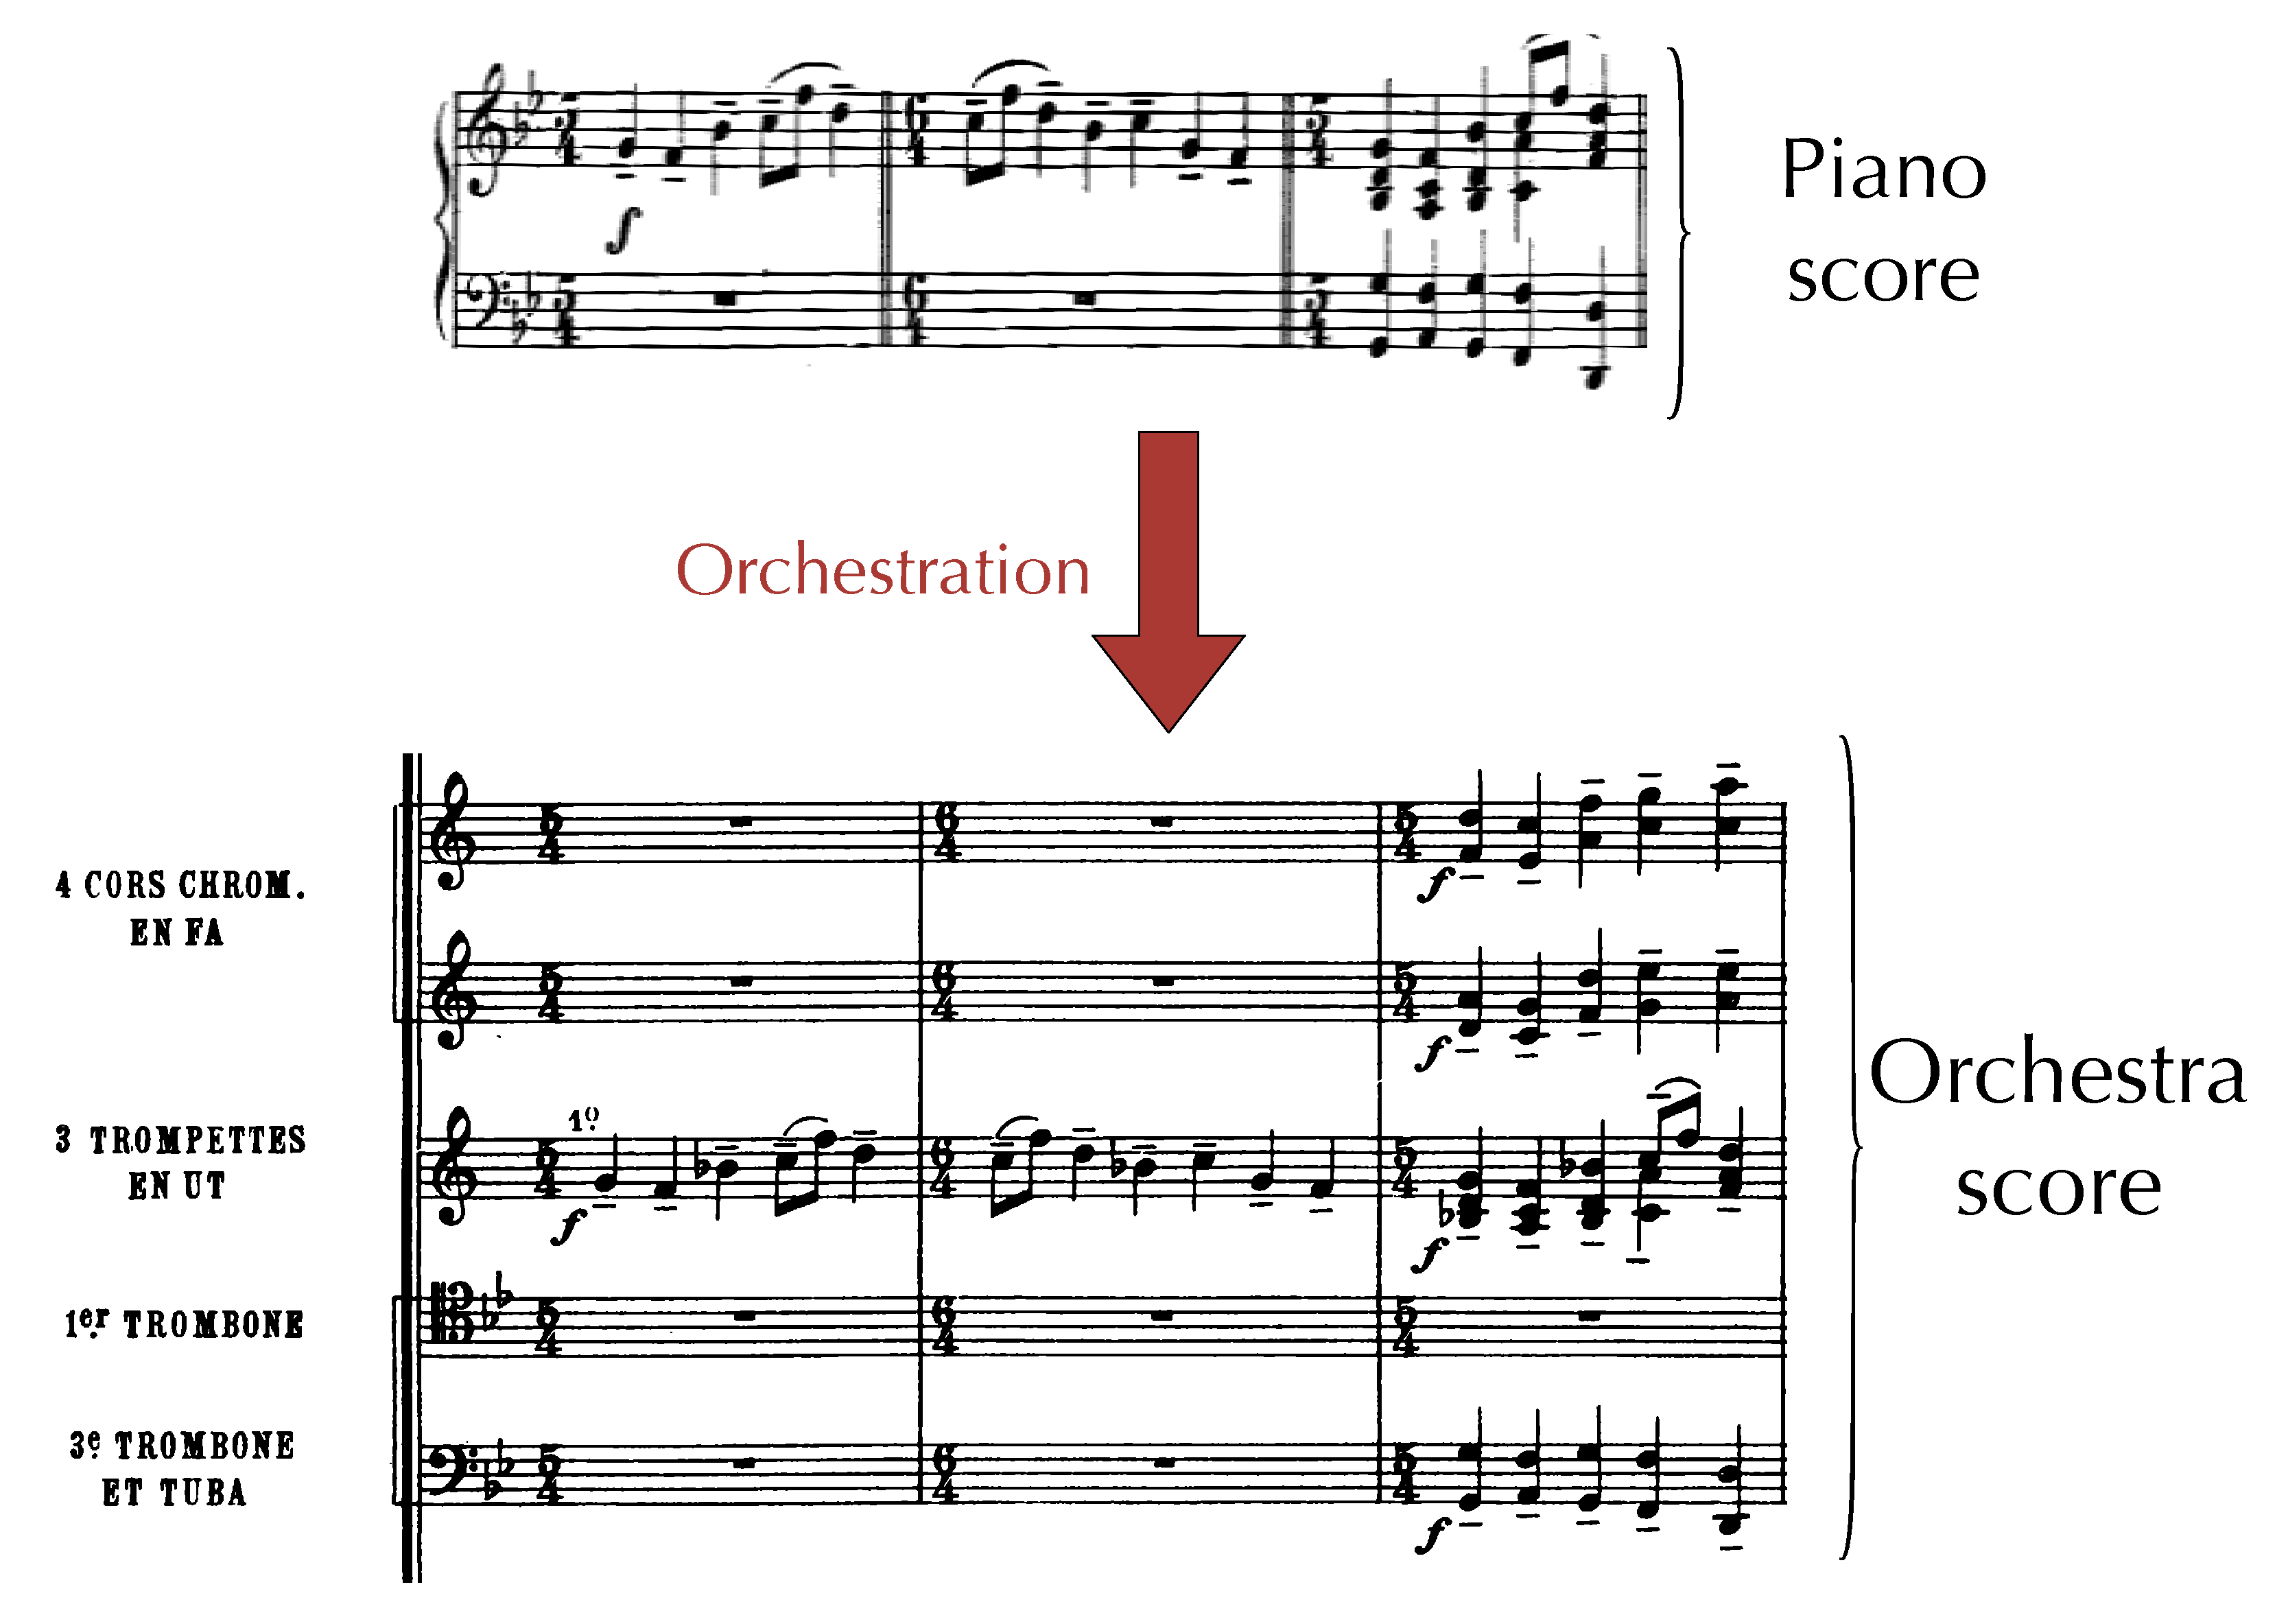
\includegraphics[scale=0.12]{orch}
\caption{\textit{Projective orchestration}. A piano score is projected on an orchestra. Even though a wide range of orchestrations exist for a given piano score, all of them will share strong relations with the original piano score. One given orchestration implicitly embeds the knowledge of the composer about timbre and orchestration.}
\label{fig:orch}
\end{figure}

% Pourquoi c'est intéressant les orchestrations projectives ?
Observing projective orchestrations made by famous composers is highly informative. First because the orchestrated version highlights the structure analyzed by the composer. Then, because it gives precious informations about the timbral mapping performed by the composer.
%
%
For these reasons, we believe that the absence of a database of projective orchestration was an acute lack to the scientific study of orchestration.

In the remainder of this paper, we introduce the database we have constructed in section 1. More specifically, we describe its structure and the alignment algorithms we used to guarantee that the piano and orchestra scores are aligned. In section 2, we introduce an task that we called \textit{automatic projective orchestration}. We then detail our approach to tackle this newly introduced problem.

%------------------------------------------------

\section{Description of the database}
\subsection{Structure}
The database is composed by \textbf{NN} pairs of piano score and their orchestration. 
Each pair has a unique index.
The scores format is midi.

Because the scores come from different sources, we had to standardize  informations. Hence, for each midi file, a comma separated values (\textit{csv}) file link the name of the midi tracks to an instrument name (exemple : \textit{pia\_001} is linked to \textit{piano}).
Besides, a 
\subsection{Automatic alignment}
Since we gathered files from various origins, we had to perform automatic alignment for each pair. We used a \textit{Needleman-Wunsch} based algorithm with a measure adapted to the musical context.
%------------------------------------------------

\section{Projective orchestration}


%----------------------------------------------------------------------------------------
%	REFERENCE LIST
%----------------------------------------------------------------------------------------

\begin{thebibliography}{99} % Bibliography - this is intentionally simple in this template

\bibitem[Figueredo and Wolf, 2009]{Figueredo:2009dg}
Figueredo, A.~J. and Wolf, P. S.~A. (2009).
\newblock Assortative pairing and life history strategy - a cross-cultural
  study.
\newblock {\em Human Nature}, 20:317--330.
 
\end{thebibliography}

%----------------------------------------------------------------------------------------

\end{document}
